% Template for Cogsci submission with R Markdown

% Stuff changed from original Markdown PLOS Template
\documentclass[10pt, letterpaper]{article}

\usepackage{cogsci}
\usepackage{pslatex}
\usepackage{float}
\usepackage{caption}

% amsmath package, useful for mathematical formulas
\usepackage{amsmath}

% amssymb package, useful for mathematical symbols
\usepackage{amssymb}

% hyperref package, useful for hyperlinks
\usepackage{hyperref}

% graphicx package, useful for including eps and pdf graphics
% include graphics with the command \includegraphics
\usepackage{graphicx}

% Sweave(-like)
\usepackage{fancyvrb}
\DefineVerbatimEnvironment{Sinput}{Verbatim}{fontshape=sl}
\DefineVerbatimEnvironment{Soutput}{Verbatim}{}
\DefineVerbatimEnvironment{Scode}{Verbatim}{fontshape=sl}
\newenvironment{Schunk}{}{}
\DefineVerbatimEnvironment{Code}{Verbatim}{}
\DefineVerbatimEnvironment{CodeInput}{Verbatim}{fontshape=sl}
\DefineVerbatimEnvironment{CodeOutput}{Verbatim}{}
\newenvironment{CodeChunk}{}{}

% cite package, to clean up citations in the main text. Do not remove.
\usepackage{cite}

\usepackage{color}

% Use doublespacing - comment out for single spacing
%\usepackage{setspace}
%\doublespacing


% % Text layout
% \topmargin 0.0cm
% \oddsidemargin 0.5cm
% \evensidemargin 0.5cm
% \textwidth 16cm
% \textheight 21cm

\title{Exploring a Causal Link between Language and Cultural Biases}


\author{{\large \bf Molly Lewis} \\ \texttt{mollyllewis@gmail.com} \\ Department of Psychology  \\ University of Wisconsin-Madison \And {\large \bf Gary Lupyan} \\ \texttt{lupyan@wisc.edu} \\ Department of Psychology  \\ University of Wisconsin-Madison}

\begin{document}

\maketitle

\begin{abstract}
The abstract.

\textbf{Keywords:}
IAT, cultural biases, gender, linguistic relativity.
\end{abstract}

\section{Introduction}\label{introduction}

\section{Study 1: Cross-cultural gender bias in
behavior}\label{study-1-cross-cultural-gender-bias-in-behavior}

We quantified the degree of gender bias in a culture using data from the
Implicit Association Task (``IAT''; Greenwald, McGhee, \& Schwartz,
1998). The IAT measures the strength of respondents' associations
between two pairs of concepts (e.g., male-career/female-family
vs.~male-family/female-career). The underlying assumption of the measure
is that concepts that are represented as more similar to each other in
the cognitive system should be easier to pair together in a behavioral
task, compared to two concepts that are relatively dissimilar. Concepts
are paired in the task by assigning them to the same response keys in a
2AFC categorization task. In the critical blocks of the task, concepts
are assigned to keys in a way that is either bias-congruent (i.e.~Key A
= male/career; Key B = female/family) or bias-incongruent (i.e.~Key A =
male/family; Key B = female/career). Participants are then presented
with a word related to one of the four concepts and asked to classify it
by responding with one of the two keys as quickly as possible. Slower
reaction times in the bias-incongruent blocks relative to the
bias-congruent blocks are interpretted as an implicit association
between the correspondings concepts (i.e.~a bias to associate male with
career, and female with family).

\subsection{Method}\label{method}

We analyzed an exisiting dataset of IAT scores collected online from a
large, culturally diverse sample (Project Implicit:
\url{https://implicit.harvard.edu/implicit/}; Nosek, Banaji, \&
Greenwald,
2002)\footnote{All analysis code can be found in an online repository: https://github.com/mllewis/IATLANG}.
Our analysis included all gender-career IAT scores collected from
respondents between 2005 and 2016 who had complete data and were located
in countries with more than 400 total respondents (\emph{N} = 773,205).
We further restricted our sample based on participants' reaction times
and errors using the same criteria described in Nosek, Banjai, and
Greenwald (2002, pg. 104). Our final sample included 664,359
participants from 49 countries, with a median of 1,123 participants per
country.

Several measures have been used in the literature to describe the
difference in reaction time between bias congruent and incongruent
blocks. Here, we use the best perfomring measure, D-score, which
quantifies the difference between critical blocks while also accounting
for individual differences in response time (Greenwald, Nosek, \&
Banaji, 2003).

In addition to the implicit measure, we also analyzed an explicit
measure of gender bias. After completing the IAT, participants were
asked, ``How strongly do you associate the following with males and
females?'' for both the words ``career'' and ``family.'' Participants
indicated their response on a Likert scale ranging from female (1) to
male (7). We calculated an explicit gender bias score for each
participant as the career response minus the family response, such that
greater values indicated more gender bias (as for the D-score).

\subsection{Results}\label{results}

\begin{CodeChunk}
\begin{figure}[t]

{\centering 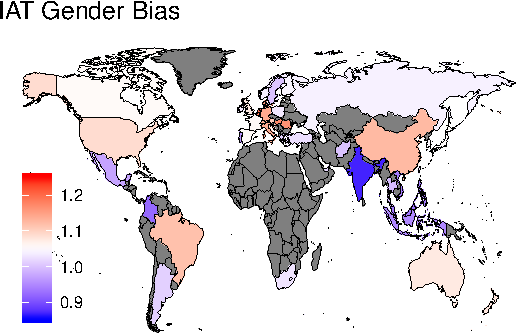
\includegraphics{figs/map-1} 

}

\caption[IAT gender bias (D-score) for the 49 countries with available data]{IAT gender bias (D-score) for the 49 countries with available data. All countries show a gender bias, with red indicating above average and blue indicating below average bias.}\label{fig:map}
\end{figure}
\end{CodeChunk}

Broadly, we replicate the patterns in the IAT literature (Nosek et al.,
2002). First, participants in all countries showed a bias to associate
men with career and females with family. Figure 1 shows the magnitude of
the IAT gender bias (D-score) across all 49 countries (\emph{M} = 0.37;
\emph{SD} = 0.03). Second, implicit and explicit bias measures were
correlated both at the level of individual participants (\emph{r} =
0.15; \emph{p} \textless{} .00001) and at the level of countries
(\emph{r} = 0.31; \emph{p} = 0.03).

Finally, previous work has shown a difference for women

\section{Study 2: Cross-cultural gender bias in
language}\label{study-2-cross-cultural-gender-bias-in-language}

In Study 2, we ask whether participants' implicit and explicit gender
biases are correlated with biases found in the semantics of
participants' native languages. To model semantics, we turn to a
recently developed machine-learning method for deriving lexical
semantics from text: auto-encoding neural network models. The underlying
assumption of these models is that the meaning of a word can be
described by the words it tends to co-occur with -- an approach known as
distributional semantics (Firth, 1957). Under this approach, a word like
``dog'' is represented more semantically similar to ``hound'' than
``banana'' because it co-occurs with words more in common with ``hound''
than ``banana'' in a large corpus of text.

Recent developments in machine learning allow for the implementation of
the idea of distributional semantics in a way that both takes into
account many features of local language structure while remaining
computationally tractable. The best known of these word embedding models
is \emph{word2vec} (Mikolov, Chen, Corrado, \& Dean, 2013). The model's
output is a vector for each word reprseneting its semantics. A measure
of the semantic similarity between two words can be derived by taking
the distance between the word vectors (using cosine distance, for
example). Similarity measures derived from these models have been shown
to be highly correlated with human judgements of word similarity (e.g.,
Hill, Reichart, \& Korhonen, 2015).

Recent work has used models like \emph{word2vec} to measure the presence
of social biases in the semantics of English in a way that is highly
analogus to the behvioral IAT (Caliskan, Bryson, \& Narayanan, 2017;
henceforth \emph{CBN}). This is done by measuring the distance in vector
space between the same sets of words that are presented to participants
in the IAT. They demonstrate that these distance measures are highly
correlated with reaction times in the behavioral IAT task, suggesting
that the biases measured by the IAT are also found in the lexical
semantics of natural language.

In Study 2, we use the method described by CBN to measure the biases in
the semantics of the natural languages spoken in the countries of
participants in Study 1. To do this, we take advantage of a set of
models that have been pre-trained on the corpus of Wikipedia text in a
large number of languages (Bojanowski, Grave, Joulin, \& Mikolov, 2016).
In Study 2a, we replicate the CBN findings with the Wikipedia corpus; In
Study 2b, we demonstrate that the implicit and explicit gender biases
reported in Study 1 for individual countries are correlated with the
biases found in the semantics of the natural language spoken by those
participants.

\subsection{Study 2a: Replication of Caliskan, et
al.~(2017)}\label{study-2a-replication-of-caliskan-et-al.2017}

\subsubsection{Method}\label{method-1}

We use a word embedding model that has been pre-trained model on the
corpus of English Wikipedia using the fastText algorithm (Bojanowski et
al.,
2016)\footnote{Available here: https://github.com/facebookresearch/fastText/}.
The model contains 2,519,370 words with each word reprsented by a 300
dimension vector.

Using the Wikpedia fastText model, we calculate an effect size for each
of the 10 biases reported in CBN, corresponding to behavioral IAT
results existing in the literature: flowers-insects,
instruments-weapons, race, gender-career gender-math, gender-science,
mental-physical (originally labeled as WEAT 1-10). We calculate the bias
using the same effect size metric described in CBN, a standardized
difference score in the relative similarity of the target words to the
target attributes (i.e.~relative similarity of male to career
vs.~relative similarity of female to career). This measure is analagous
the behavioral D-score measure in Study 1 and, like for D-score, larger
values indicate a larger bias.

\subsubsection{Results}\label{results-1}

\begin{CodeChunk}
\begin{figure}[t]

{\centering 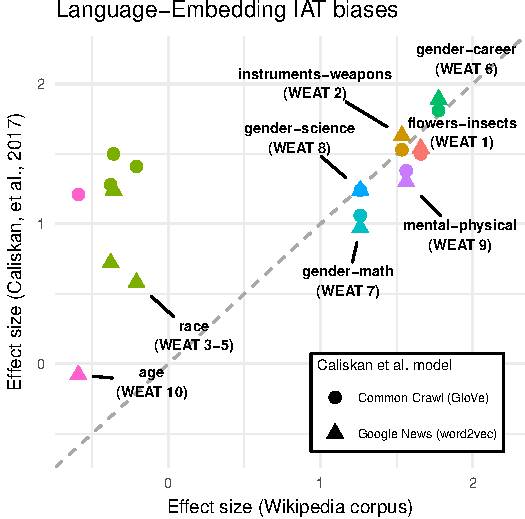
\includegraphics{figs/WEAT_plot-1} 

}

\caption[Effect sizes for the 10 IAT biases types (WEAT 1-10) reported in Caliskan et al]{Effect sizes for the 10 IAT biases types (WEAT 1-10) reported in Caliskan et al. (2017; CBN). The effect sizes reported in CBN are plotted against  effect sizes from the Wikipedia corpus.  Color corresponds to  bias type, and shape corresponds to the two CBN models trained on different corpora and with different algorithms.}\label{fig:WEAT_plot}
\end{figure}
\end{CodeChunk}

Figure 2 shows the effect size measures derived from the Wikipedia
corpus plotted against effect size esimtates reported by CBN from two
different models (trained on the Common Crawl and Google News corpora).
With the exception of biases related to race and age, effect sizes from
the Wikipedia corpus are highly similar to those reported by CBN. In
particular, for the gender-career IAT -- the bias relevant to our
current purposes -- we estimate the effect size to be 1.78, and CBN
estimates it to be 1.81 (Common Crawl) and 1.89 (Google News).

\subsection{Study 2b: Predicting implicit bias with language
IAT}\label{study-2b-predicting-implicit-bias-with-language-iat}

With our corpus validated, we next turn to estimating the magnitude of
the gender-career bias in the each of the languages spoken in the
countries described in Study 1 with the goal of examining the
relationship between behavioral gender biases and language gender
biases.

\subsubsection{Method}\label{method-2}

\subsubsection{Results}\label{results-2}

\section{Study 3: grammar and bias}\label{study-3-grammar-and-bias}

\section{Study 4: exploring bias more
directly}\label{study-4-exploring-bias-more-directly}

\section{Conclusion}\label{conclusion}

\section{References}\label{references}

\setlength{\parindent}{-0.1in} \setlength{\leftskip}{0.125in} \noindent

\hypertarget{refs}{}
\hypertarget{ref-bojanowski2016enriching}{}
Bojanowski, P., Grave, E., Joulin, A., \& Mikolov, T. (2016). Enriching
word vectors with subword information. \emph{arXiv Preprint
arXiv:1607.04606}.

\hypertarget{ref-caliskan2017semantics}{}
Caliskan, A., Bryson, J. J., \& Narayanan, A. (2017). Semantics derived
automatically from language corpora contain human-like biases.
\emph{Science}, \emph{356}(6334), 183--186.

\hypertarget{ref-firth1957synopsis}{}
Firth, J. (1957). A synopsis of linguistic theory 1930-1955 in studies
in linguistic analysis, philological society. Oxford. reprinted in
Palmer, F.,(ed. 1968), Selected Papers of JR Firth, Longman, Harlow.

\hypertarget{ref-greenwald1998measuring}{}
Greenwald, A. G., McGhee, D. E., \& Schwartz, J. L. (1998). Measuring
individual differences in implicit cognition: The implicit association
test. \emph{Journal of Personality and Social Psychology}, \emph{74}(6),
1464.

\hypertarget{ref-greenwald2003understanding}{}
Greenwald, A. G., Nosek, B. A., \& Banaji, M. R. (2003). Understanding
and using the implicit association test: I. an improved scoring
algorithm. \emph{Journal of Personality and Social Psychology},
\emph{85}(2), 197.

\hypertarget{ref-hill2015simlex}{}
Hill, F., Reichart, R., \& Korhonen, A. (2015). Simlex-999: Evaluating
semantic models with (genuine) similarity estimation.
\emph{Computational Linguistics}, \emph{41}(4), 665--695.

\hypertarget{ref-mikolov2013efficient}{}
Mikolov, T., Chen, K., Corrado, G., \& Dean, J. (2013). Efficient
estimation of word representations in vector space. \emph{arXiv Preprint
arXiv:1301.3781}.

\hypertarget{ref-nosek2002harvesting}{}
Nosek, B. A., Banaji, M. R., \& Greenwald, A. G. (2002). Harvesting
implicit group attitudes and beliefs from a demonstration web site.
\emph{Group Dynamics: Theory, Research, and Practice}, \emph{6}(1), 101.

\end{document}
